\documentclass[compress,red]{beamer}
\mode<presentation>
\setbeamertemplate{navigation symbols}{}

\usetheme{Warsaw}
% other themes: AnnArbor, Antibes, Bergen, Berkeley, Berlin, Boadilla, boxes, CambridgeUS, Copenhagen, Darmstadt, default, Dresden, Frankfurt, Goettingen,
% Hannover, Ilmenau, JuanLesPins, Luebeck, Madrid, Maloe, Marburg, Montpellier, PaloAlto, Pittsburg, Rochester, Singapore, Szeged, classic

%\usecolortheme{lily}
% color themes: albatross, beaver, beetle, crane, default, dolphin, dov, fly, lily, orchid, rose, seagull, seahorse, sidebartab, structure, whale, wolverine

%\usefonttheme{serif}
% font themes: default, professionalfonts, serif, structurebold, structureitalicserif, structuresmallcapsserif

\hypersetup{pdfpagemode=FullScreen} % makes your presentation go automatically to full screen

% define your own colors:
\definecolor{Red}{rgb}{1,0,0}
\definecolor{Blue}{rgb}{0,0,1}
\definecolor{Green}{rgb}{0,1,0}
\definecolor{magenta}{rgb}{1,0,.6}
\definecolor{lightblue}{rgb}{0,.5,1}
\definecolor{lightpurple}{rgb}{.6,.4,1}
\definecolor{gold}{rgb}{.6,.5,0}
\definecolor{orange}{rgb}{1,0.4,0}
\definecolor{hotpink}{rgb}{1,0,0.5}
\definecolor{newcolor2}{rgb}{.5,.3,.5}
\definecolor{newcolor}{rgb}{0,.3,1}
\definecolor{newcolor3}{rgb}{1,0,.35}
\definecolor{darkgreen1}{rgb}{0, .35, 0}
\definecolor{darkgreen}{rgb}{0, .6, 0}
\definecolor{darkred}{rgb}{.75,0,0}

\xdefinecolor{olive}{cmyk}{0.64,0,0.95,0.4}
\xdefinecolor{purpleish}{cmyk}{0.75,0.75,0,0}

% can also choose different themes for the "inside" and "outside"

% \usepackage{beamerinnertheme_______}
% inner themes include circles, default, inmargin, rectangles, rounded

% \usepackage{beamerouterthemesmoothbars}
% outer themes include default, infolines, miniframes, shadow, sidebar, smoothbars, smoothtree, split, tree

\useoutertheme[subsection=false]{smoothbars}

% to have the same footer on all slides
%\setbeamertemplate{footline}[text line]{STUFF HERE!}
%\setbeamertemplate{footline}[text line]{} % makes the footer EMPTY
\setbeamertemplate{footline}[page number]

% include packages
\usepackage{subfigure}
\usepackage{multicol}
\usepackage{amsmath}
\usepackage{epsfig}
\usepackage{graphicx}
%\usepackage[all,knot]{xy}
%\xyoption{arc}
\usepackage{url}
\usepackage{multimedia}
\usepackage{hyperref}
\usepackage{helvet}
\usepackage[polish,english]{babel}
\usepackage[utf8]{inputenc}
\usepackage{eurosym}

% greetings, introduce yourself

\title[WR Project Status\hspace{2em}\insertframenumber/
\inserttotalframenumber]{The White Rabbit Project}

\subtitle{Technical introduction and status report}
\author{Erik van der Bij, Pablo \'A{}lvarez, Evangelia Gousiou,\\Maciej
  Lipi\'{n}ski, Javier Serrano, Tomasz W\l{}ostowski}
\date{November 29, 2011}

\institute%[Universities of Somewhere and Elsewhere] % (optional, but mostly needed)
{
  BE-CO Hardware and Timing section\\
  CERN, Geneva, Switzerland
 }

\pgfdeclareimage[height=0.5cm]{wr-logo}{wr-logo.jpg}
\logo{\pgfuseimage{wr-logo}}
\AtBeginSection[]
{
  \begin{frame}<beamer>{Outline}
    \tableofcontents[currentsection]
  \end{frame}
}

\begin{document}

\frame{\titlepage}

% wr is a multilab, multicompany project which aim is to build next-gen control&timing network based on ethernet.

\section{Introduction}

\subsection{}

\begin{frame}{BE-CO-HT mission}
\begin{block}{Provide HW kit for equipment groups at CERN}
Based on carriers (VME64x, PCIe\ldots) and FMC (VITA 57) mezzanines.
\end{block}
\begin{block}{Act as knowledge hub for hardware design}
FPGA designs based on Wishbone bus, ADC, DAC, TDC, fine delay generators\ldots
\end{block}
\begin{block}{Provide low-level software support for the HW kit}
Linux device drivers and libraries, production testing environment\ldots
\end{block}
\begin{block}{Design and operate CERN's General Machine
    Timing system}
Based on the HW and SW technologies the section develops. We eat our
own dog food!
\end{block}
\end{frame}

\begin{frame}{Why we use Open Hardware}
\begin{block}{Get a design just the way we want it}
We fully specify the design.
\end{block}
\begin{block}{Peer review}
Get your design reviewed by experts all around the world, including companies!
\end{block}
\begin{block}{Design re-use}
When it's Open, people are more likely to re-use it.
\end{block}
\begin{block}{Healthier relationship with companies}
No vendor-locked situations. Companies selected solely on the basis of
technical excellence, good support and price.
\end{block}
\end{frame}

\begin{frame}{Example of a carrier: the SPEC board}
\begin{center}
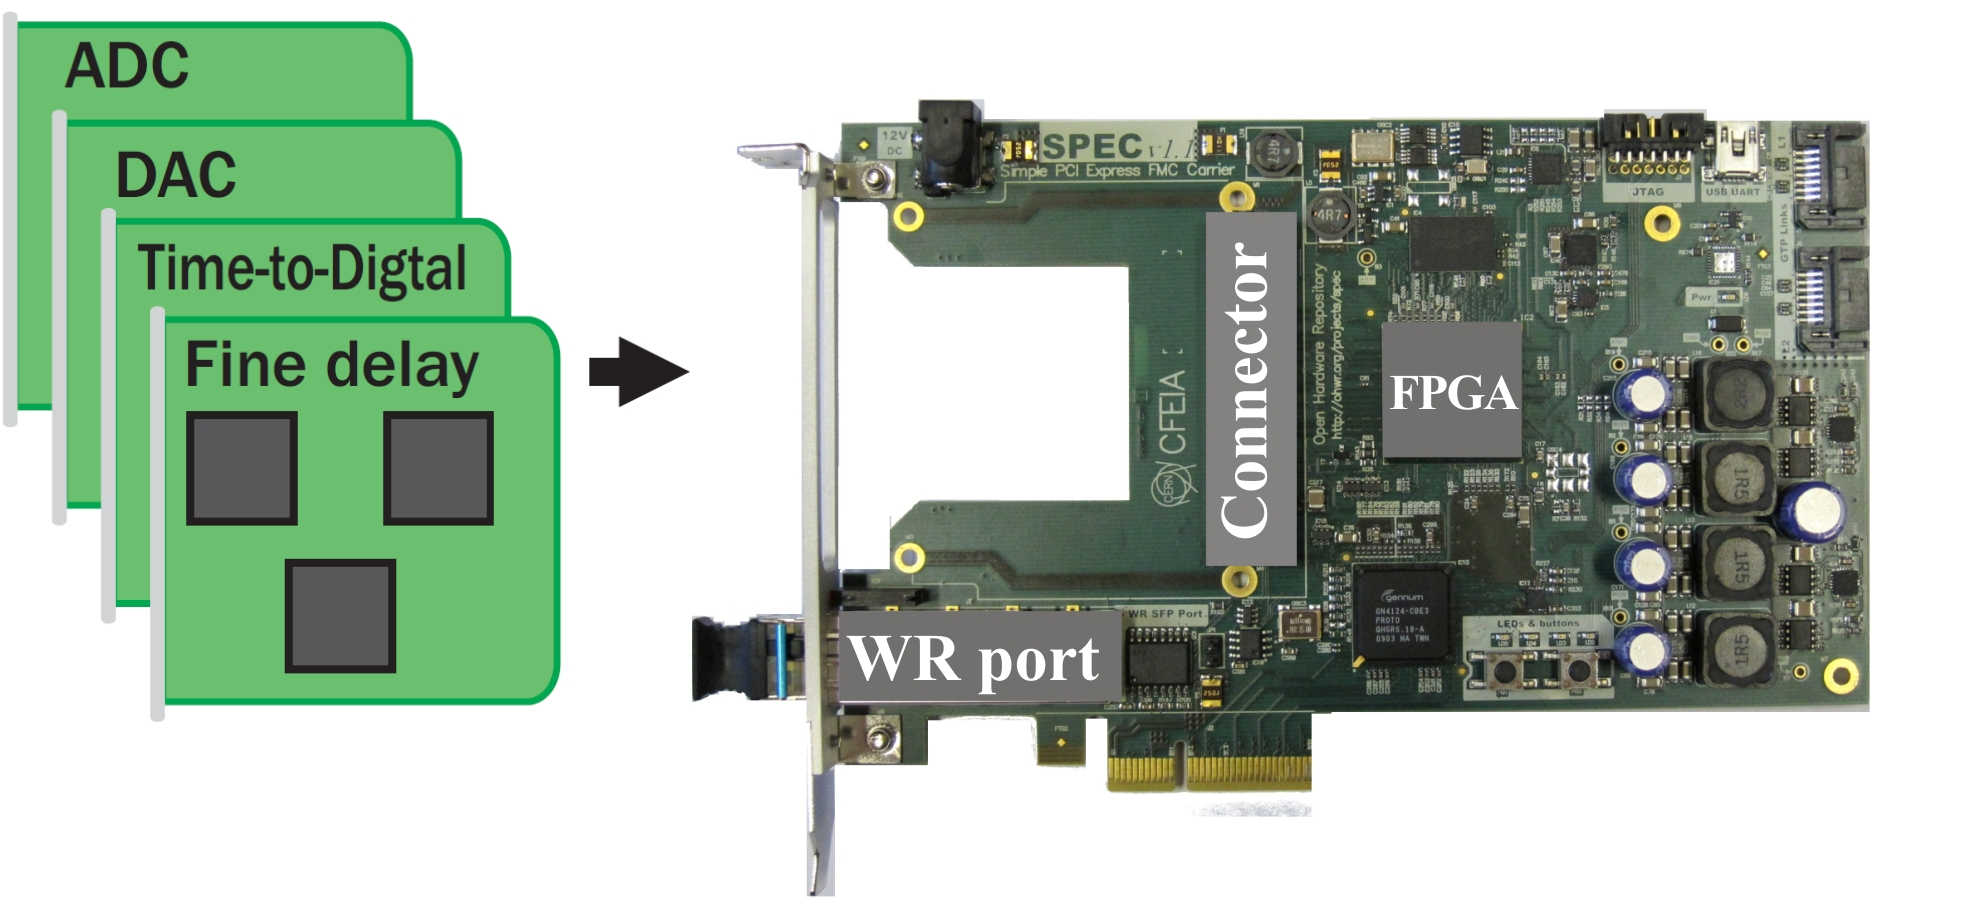
\includegraphics[height=5cm]{drawings/spec.jpg}
\begin{itemize}
\item Low-cost PCI-Express Carrier
\item Spartan-6 FPGA (XC6SLX45T), 256 MB DDR3 RAM
\item White Rabbit Ethernet port
\end{itemize}
\end{center}
\end{frame}

\begin{frame}{Example of a mezzanine: 4-channel 100MS/s ADC}
\begin{center}
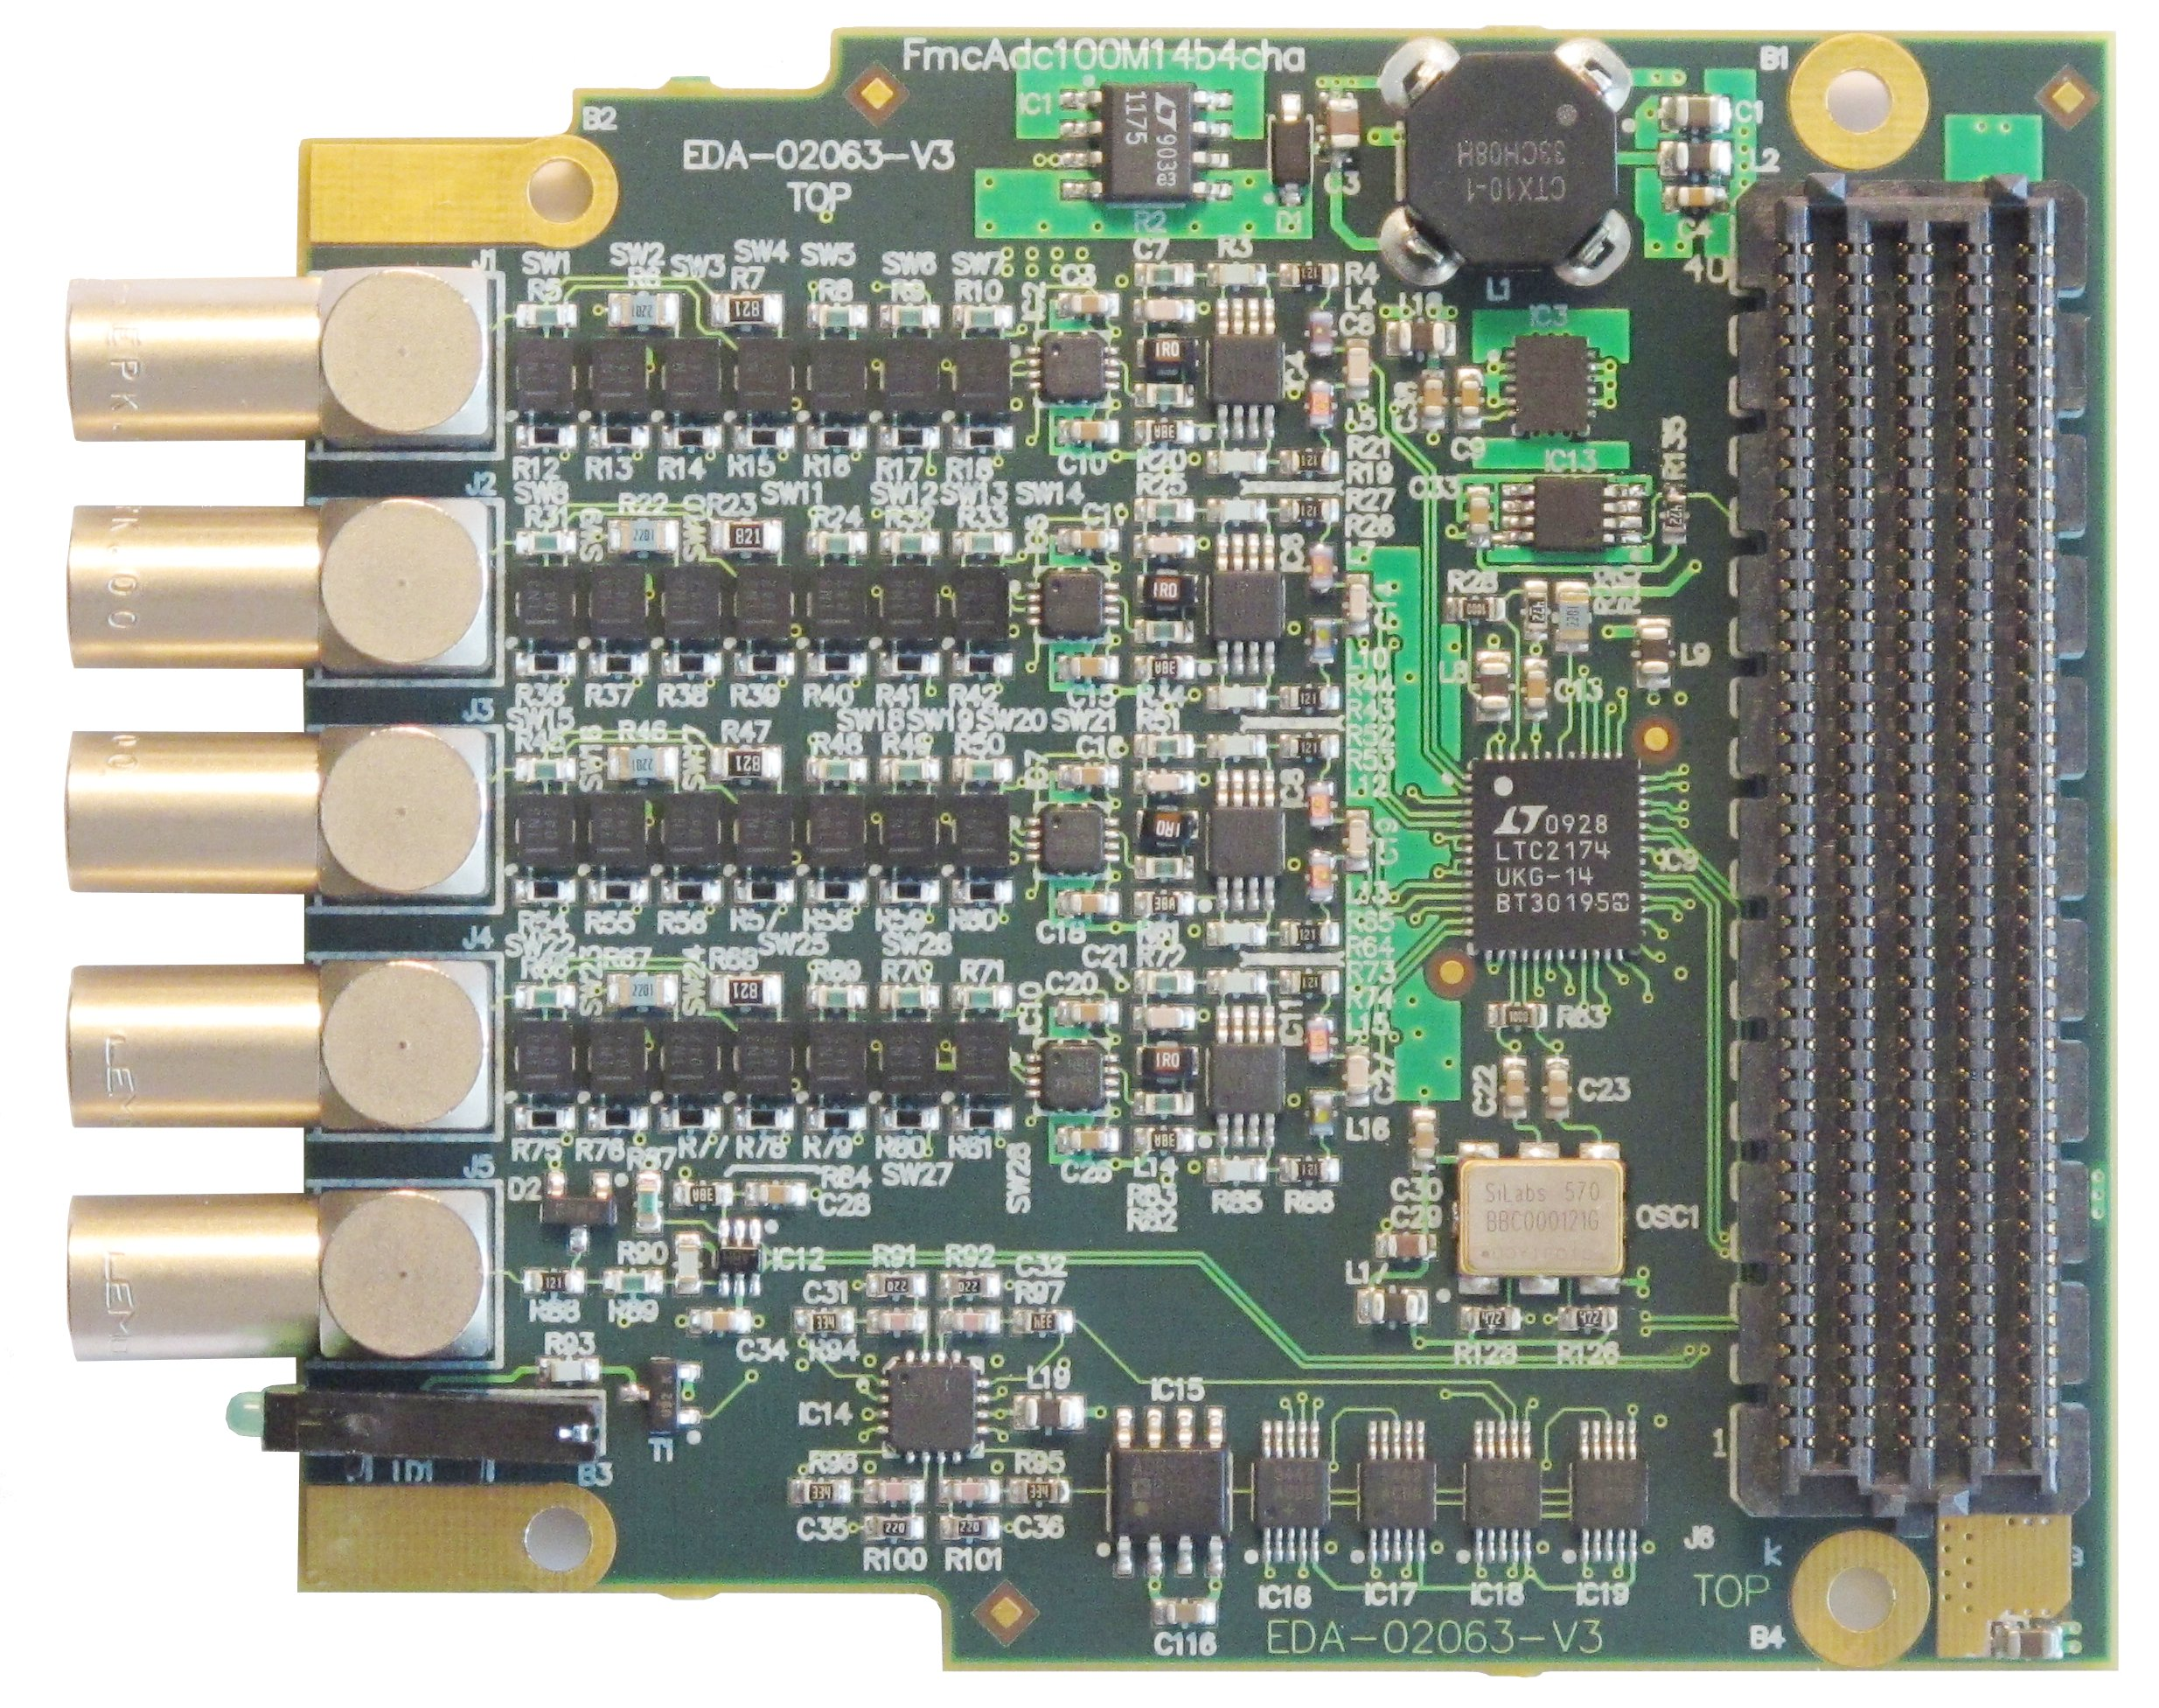
\includegraphics[height=5cm]{drawings/adc.jpg}
\begin{itemize}
\item 105 MSa/s, 14 bits (11.7 ENOB)
\item 3 input ranges ($\pm5V$, $\pm0.5V$, $\pm50mV$)
\item Flexible triggering: (external, internal or via White Rabbit)
\end{itemize}
\end{center}
\end{frame}


% Layer 2 and it's for free - transparent. Data, synchronism, determinism
% \begin{frame}{What's in a name?}
% \begin{center}
% 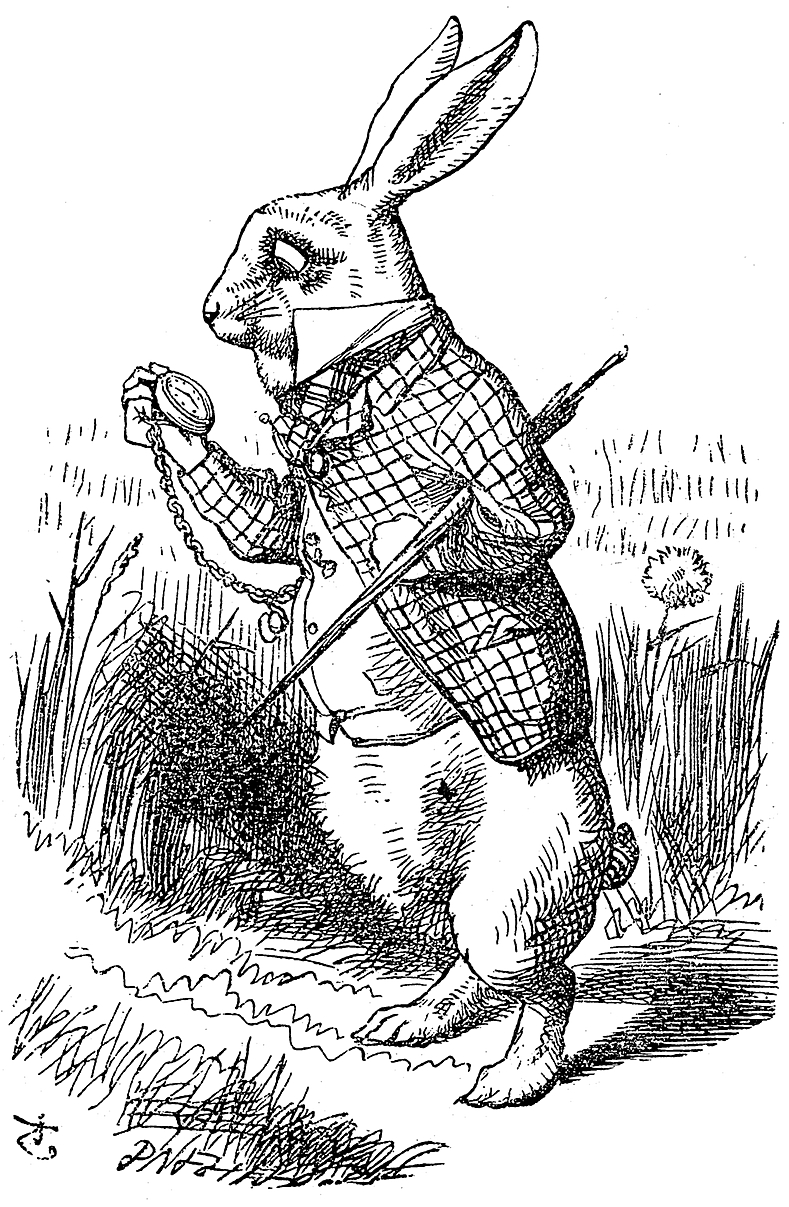
\includegraphics[height=5cm]{drawings/Alice-wr.jpg}

% \textit{Oh dear! Oh dear! I shall be too late!}\\
% \end{center}
% \end{frame}

\begin{frame}{Development model}
\begin{itemize}
\item Developed in the frame of CERN's (and GSI's) renovation projects.
\item Open source design done in collaboration with industry.
\item Commercial production and support.
\end{itemize}
\end{frame}

\begin{frame}{What is White Rabbit?}
\begin{center}
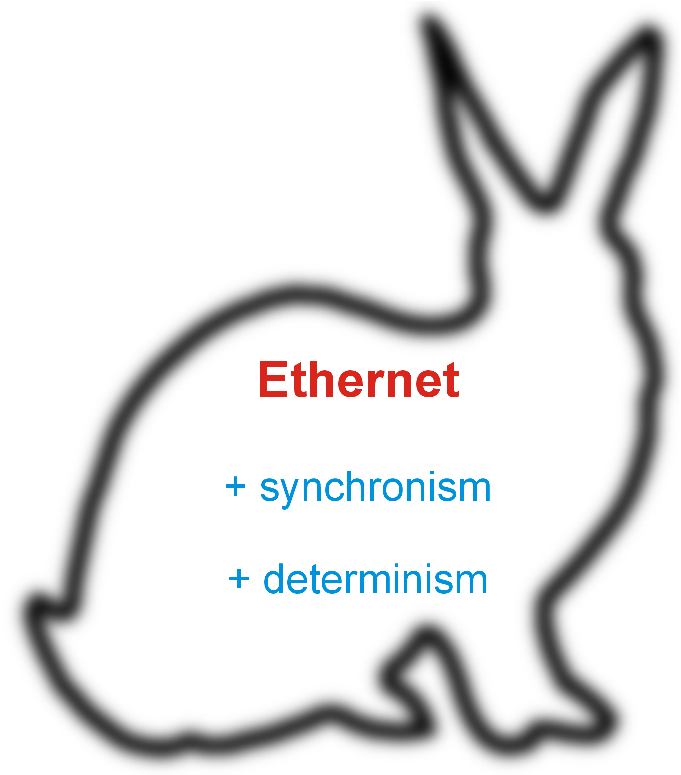
\includegraphics[height=6.5cm]{drawings/rabbit.png}
\end{center}
\end{frame}

\frame
{
  \frametitle{What is White Rabbit?}

% Extracting the clock from Ethernet carrier
\begin{block}{}
  An \textbf{extension} to \textbf{Ethernet} which provides:
  \begin{itemize}
% sync mode: - async & sync comparison, tree structure, common clock coming from single source, CDR
% advantage - easy  and precise implementation of time sync
  \item \textbf{Synchronous mode} (Sync-E) - common clock for physical layer in entire network, allowing for precise time and frequency transfer.

\item \textbf{Deterministic routing} latency - a guarantee that packet transmission delay between two stations will never exceed a certain boundary.
\end{itemize}
\end{block}

}

\begin{frame}{Design goals}
\begin{block}{Precision}
1 ns time synchronization accuracy, 20 ps jitter
\end{block}
\begin{block}{Range}
10 km fiber links
\end{block}
\begin{block}{Scalability}
Up to 2000 nodes
\end{block}
\end{frame}

\section{Technology overview}
\subsection{}
\frame{
  \frametitle{Technologies used in White Rabbit}
  Sub-nanosecond synchonization in WR is achieved by using the following three technologies together:
  \begin{itemize}
  \item Precision Time Protocol (IEEE1588)
  \item Synchronous Ethernet
  \item DMTD phase tracking
\end{itemize}
}

\frame{
\frametitle {Network topology}
% data traffic - no hierarchy, timing traffic - hierarchy	
\begin{center}
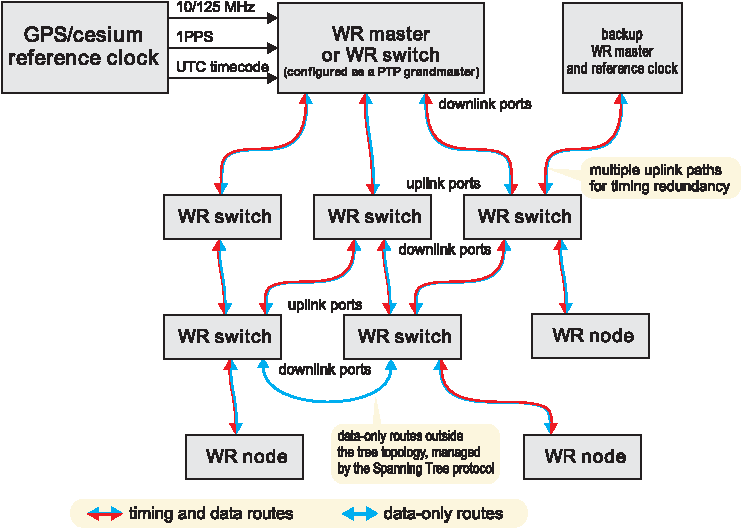
\includegraphics[height=6cm]{drawings/hierarchy.pdf}
\end{center}
}

\subsection{Precision Time Protocol (IEEE1588)}
\frame{
\frametitle{PTP Protocol (IEEE1588)}
\begin{block}{PTP}
Synchronizes local clock with the master clock by measuring and compensating the delay introduced by the link.
\end{block}

\begin{block}{Packet timestamping}
Link delay is measured by exchanging packets with precise hardware transmit/receive timestamps.
\end{block}
}

% \frame{
% \frametitle{PTP Protocol (IEEE1588)}
% \begin{columns}[c]
% \column{1.5in}
% \begin{center}
% 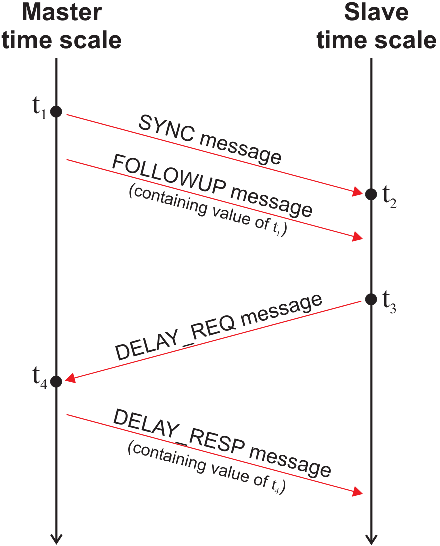
\includegraphics[height=5cm]{drawings/ptp_exchange.pdf}
% \end{center}
% \column{2.5in}
% Having values of $t_{1}...t_{4}$, slave can:
% \begin{itemize}
% \item calculate one-way link delay: $\delta_{ms} = \frac{(t_{4}-t_{1}) - (t_{3}-t_{2})}{2}$
% \item syntonize its clock rate with the master by tracking the value of $t_{2} - t_{1}$
% \item compute clock offset: $offset = t_{2} - t_{1} + \delta_{ms}$
% \end{itemize}
% \end{columns}
% }

\frame{
\frametitle{Disadvantages of traditional PTP}
  \begin{itemize}
    \item 
      All nodes have free-running oscillators.
    \item
      Frequency drift has to be continously compensated, causing lots of network traffic.
    \item
      That doesn't go well with determinism...
  \end{itemize}
}

% Extracting clock from the data - timing idea applied to network.
% gigabit PHYs - easy to get good quality clock
\subsection{Synchronous Ethernet}
% \frame{
%   \frametitle {Synchronous Ethernet}
	
%   \begin{block}{Common clock for the entire network}
%     \begin{itemize}
% 	 \item All network nodes use the same physical layer clock, generated by the System Timing Master.
%          \item Clock is encoded in the Ethernet carrier and recovered by the receiver chip (PHY).
%          \item PTP is used only for compensating clock offset.
%          \item Having the same clock frequency everywhere enables phase detector technology as the means of measuring time.
%          \end{itemize}
%        \end{block}
% }

\frame{
\frametitle {Synchronous Ethernet}
\begin{center}
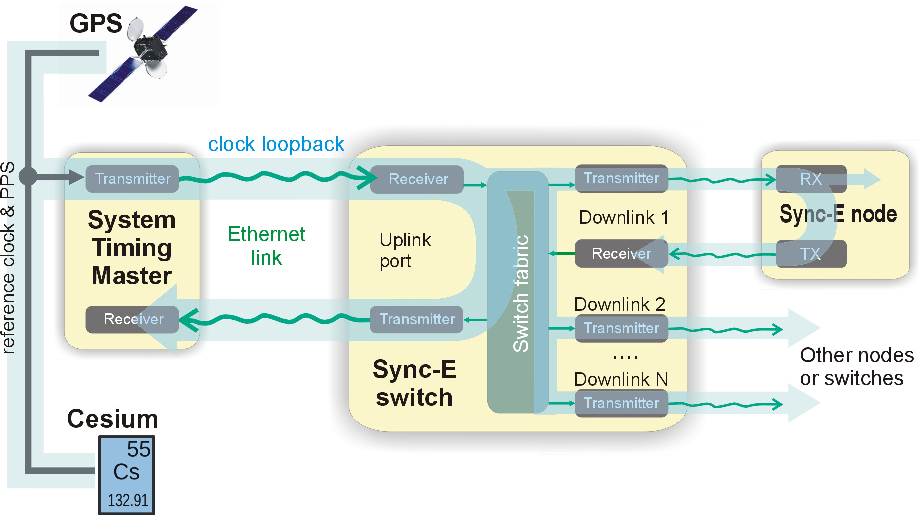
\includegraphics[height=6cm]{drawings/synce.png}
\end{center}
}

\subsection{Phase tracking}
% \frame{
% \frametitle{Phase tracking}
% \begin{block}{Plain PTP}
% PTP alone is not enough if we want very good accuracy, because of the granularity of the timestamps.
% \end{block}


% \begin{block}{Solution}
% Measure the phase shift between transmit and receive clock on the master side, taking the advantage of Synchronous Ethernet.
% \end{block}
% }

\frame{
\frametitle {Phase tracking}

\begin{center}
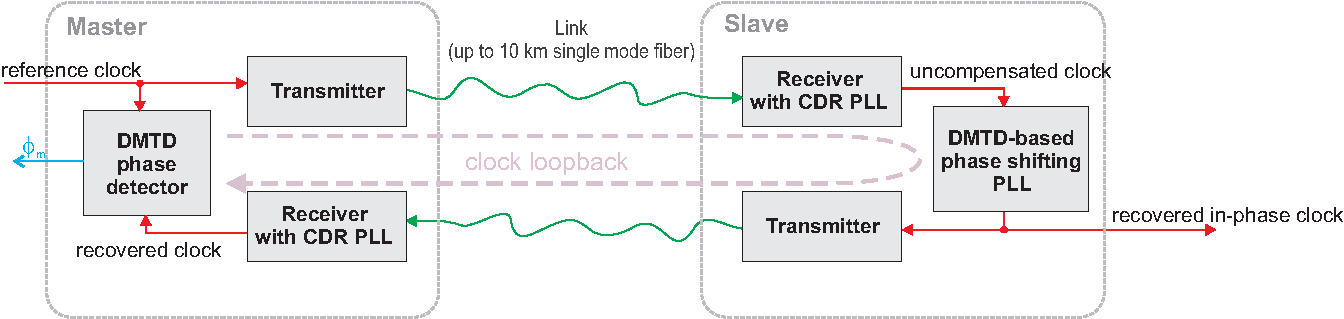
\includegraphics[height=2.5cm]{drawings/phase_tracking.pdf}
\end{center}

\begin{itemize}
\item
  Monitor phase of bounced-back clock continuously.
\item
  Phase-locked loop in the slave follows the phase changes measured by the master.
\end{itemize}
}


% \begin{frame}{Digital Dual Mixer Time Domain (DMTD) phase detector}
% \begin{center}
% 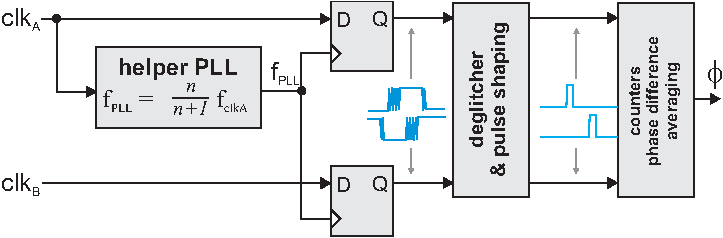
\includegraphics[width=\columnwidth]{drawings/dmtd.pdf}
% \end{center}
% \begin{itemize}
% \item Fully digital, so fully linear
% \item In a loop, it becomes a linear phase shifter
% \item Can handle multiple channels without need for extra hardware
% \end{itemize}
% \end{frame}



%\begin{frame}{Dealing with link asymmetry}
%  \begin{columns}[c]
%    \column{2in}
%    \begin{center}
%      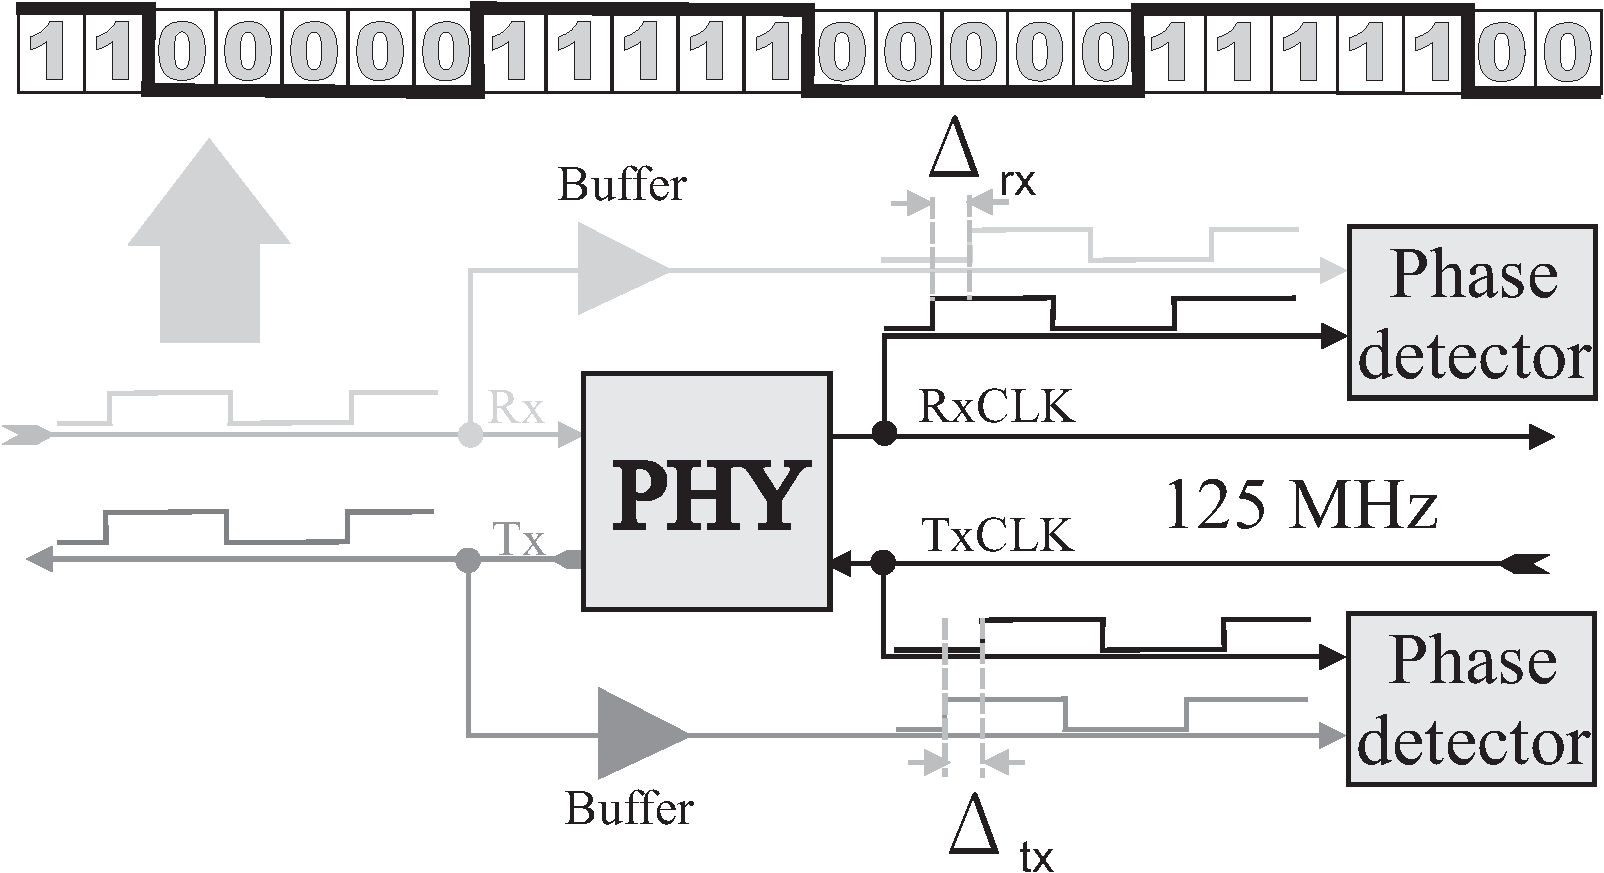
\includegraphics[height=3cm]{calibration.png}
%    \end{center}
%    PHY TX/RX latencies differ between each power-up cycle, but they can be measured using a DMT%D and a crosspoint switch.
%    \column{2in}

%    \begin{center}
%      \includegraphics[height=1.7cm]{model.png}
%    \end{center}
%    Fiber delay asymmetry is caused by difference in wavelengths for upstream and downstream tra%ffic and it increases linearly with link length.
%  \end{columns}
%\end{frame}


% \begin{frame}{What is Robustness in WR?}
% \begin{columns}[c]
%   \column{.47\textwidth}

%     \begin{block}{\center Robustness}
%       \begin{center}
% 	preventing degradation of parameters in abnormal circumstances
%       \end{center}
%     \end{block}

%   \vspace{0.2cm}

%   \begin{itemize}
%     \item \color{blue!90}{Sub-nanosecond time synchronization}
%     \item \color{red}{Deterministic Control Data delivery}
%   \end{itemize}

%   \column{.6\textwidth}
%     \begin{center}
%     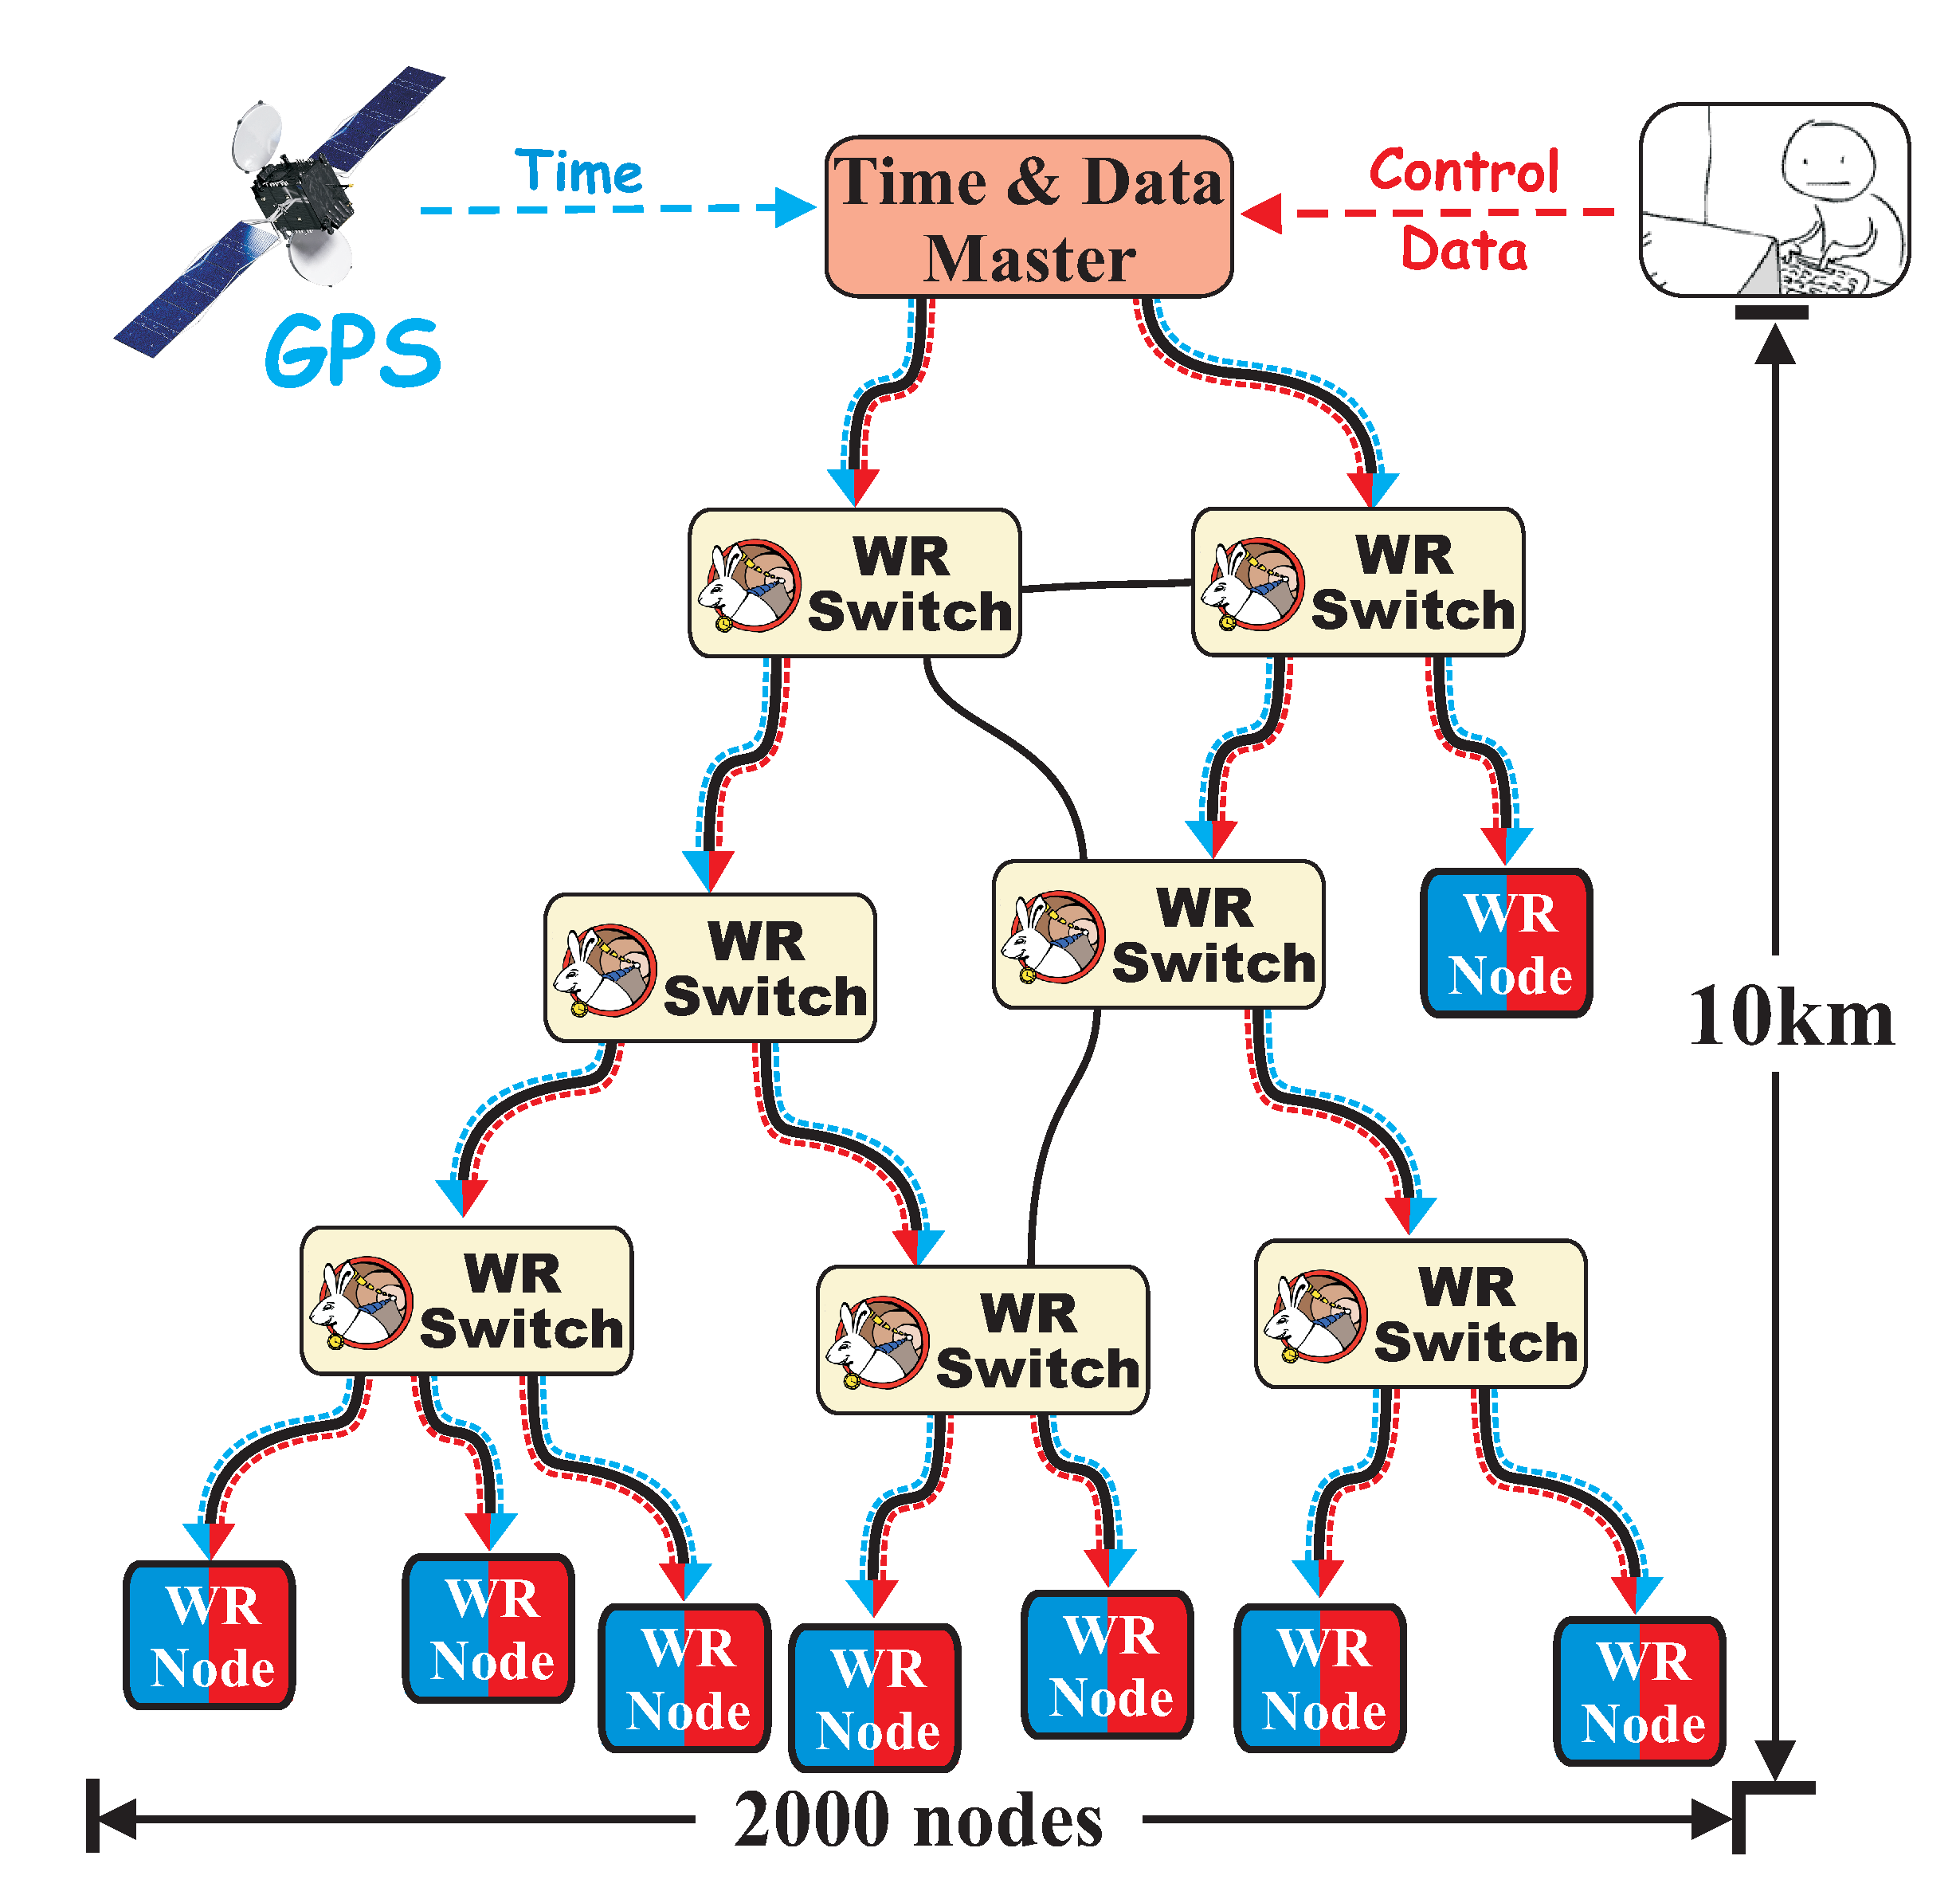
\includegraphics[height=1.0\textwidth]{drawings/wr_network-new.pdf}
%     \end{center}
% \end{columns}
% \end{frame}

% \begin{frame}{Synchronization redundancy support}

%     \begin{center}
%     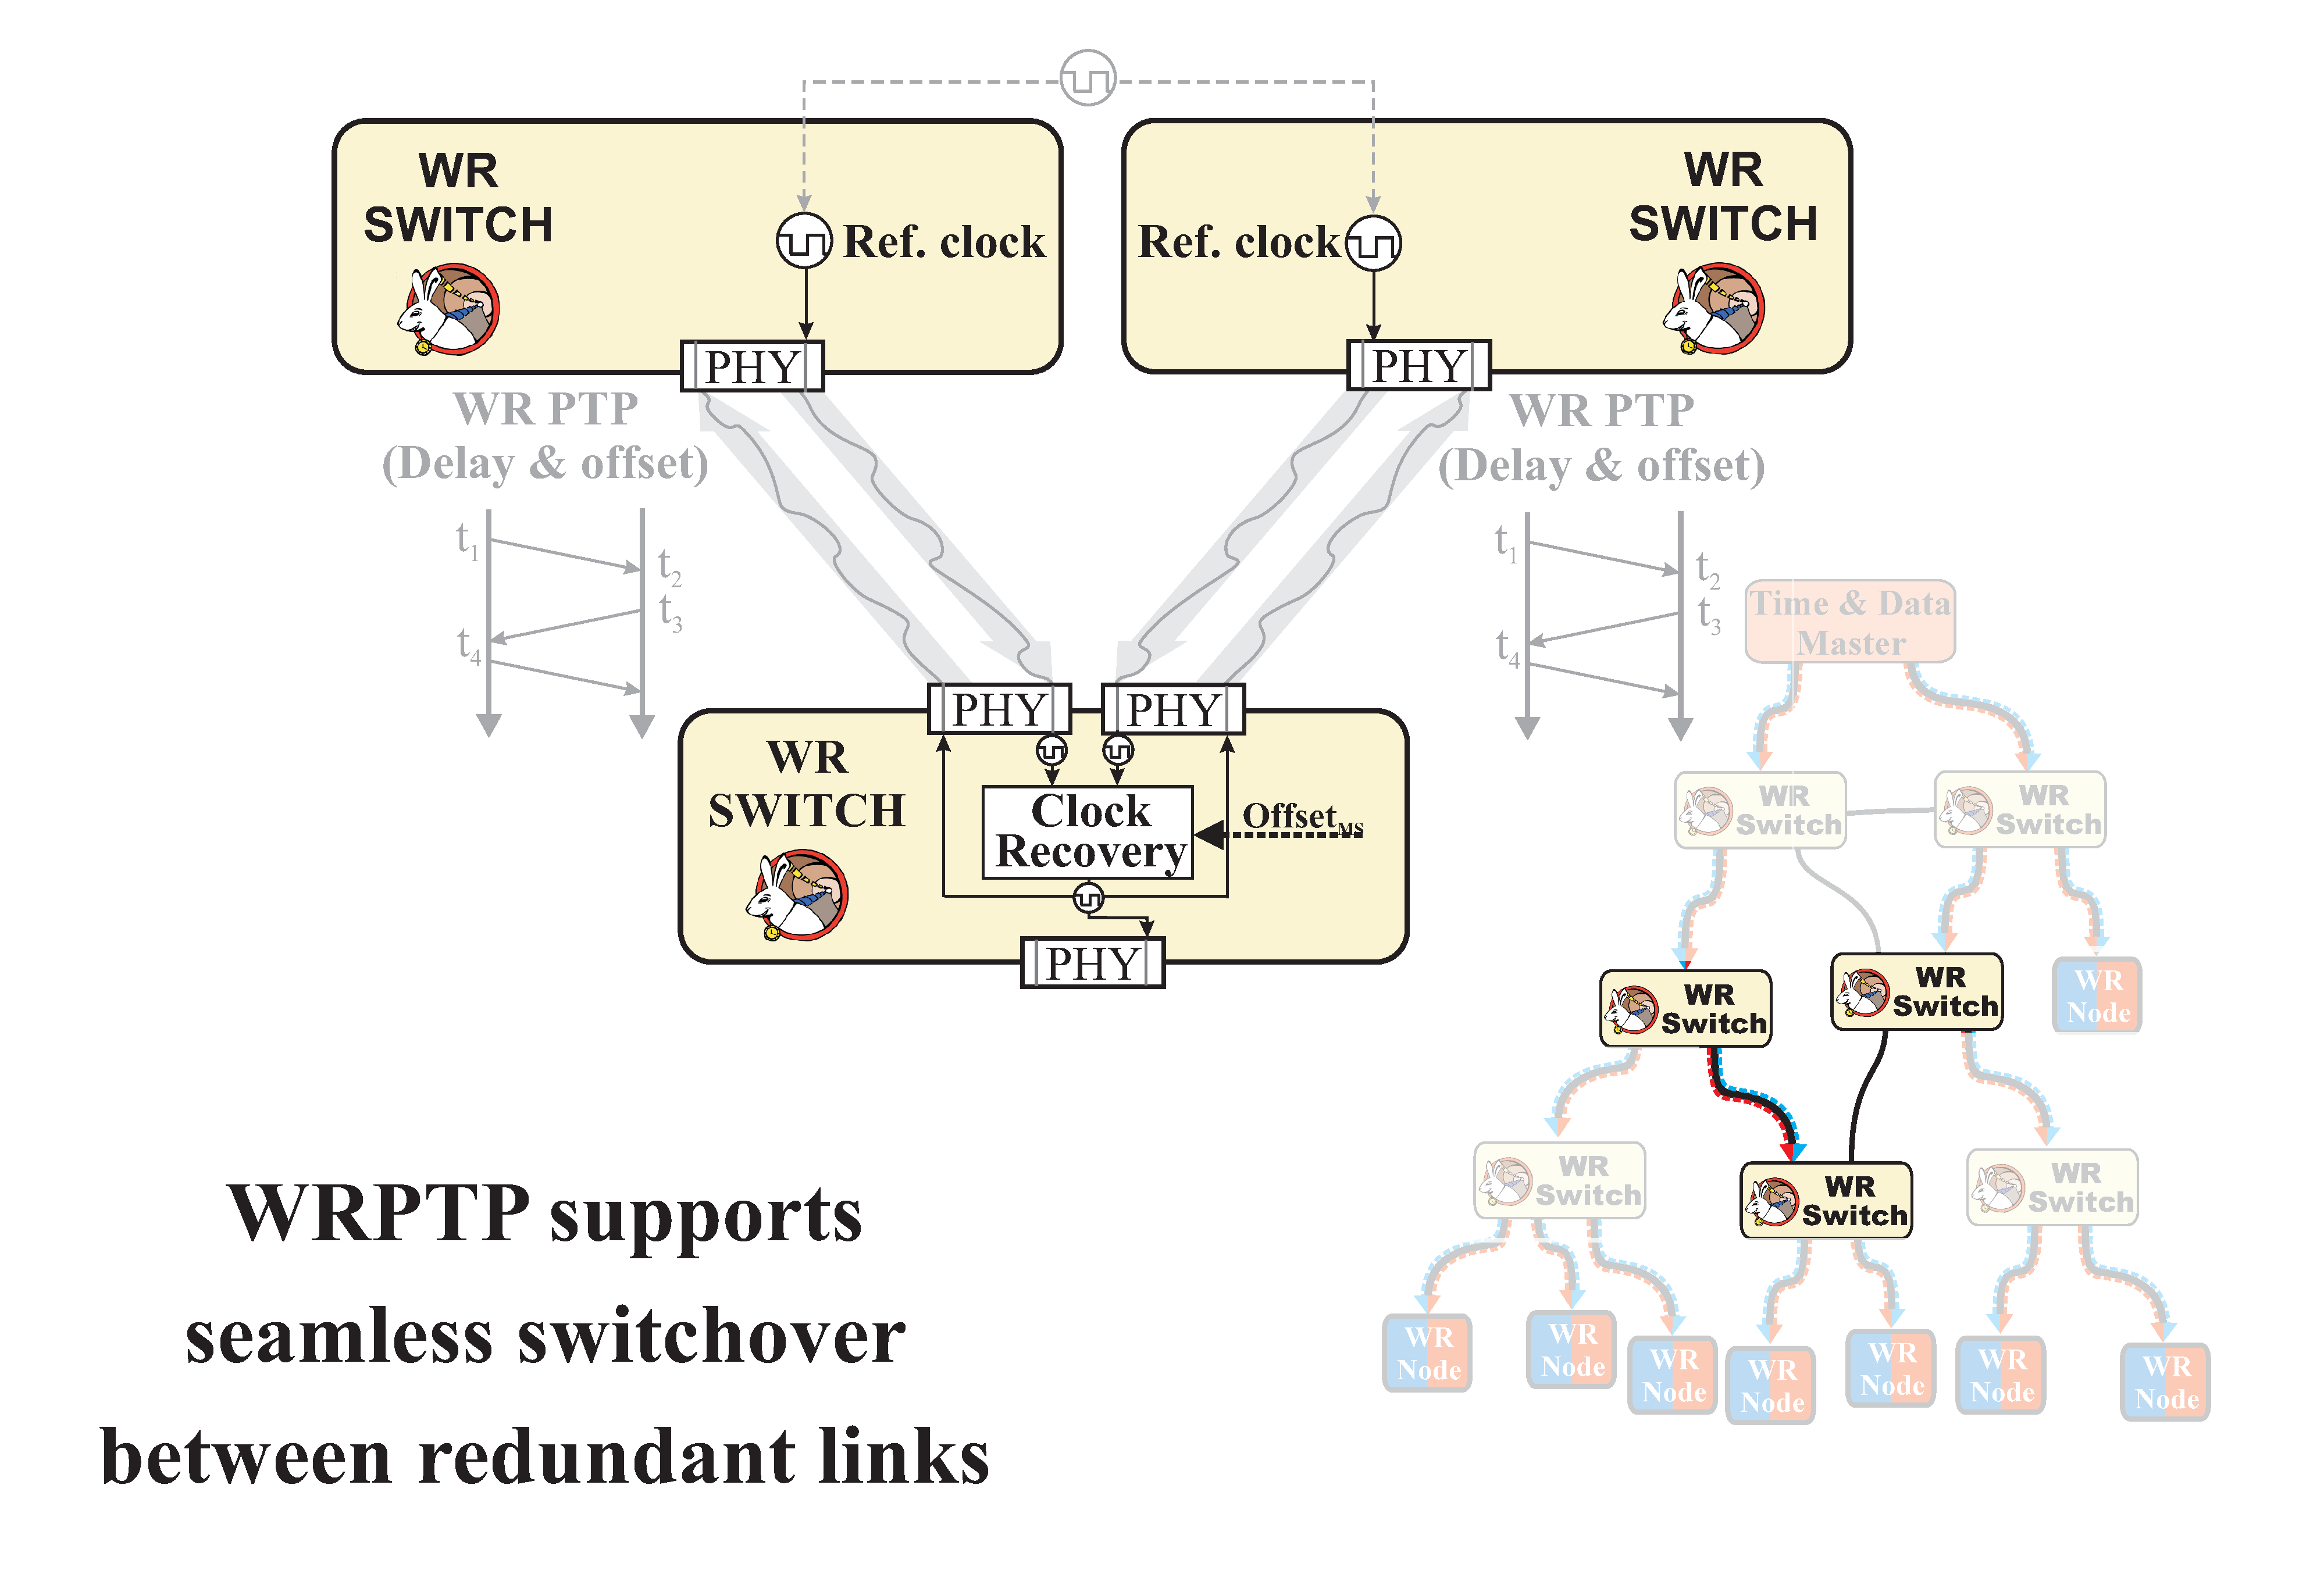
\includegraphics[width=0.9\textwidth]{drawings/wrCRS2.pdf}
%     \end{center}

% \end{frame}

\subsection {White Rabbit Switch}


\begin{frame}{White Rabbit Switch}
\begin{center}
\includegraphics[width=6.5cm]{drawings/wrs_photo.jpg}
\end{center}
\begin{itemize}
\item Central element of WR network
\item Fully custom design, done from scratch at CERN
\item Ten 1000Base-X ports, may drive 10+ km of SM fiber
\item 200 ps synchronization accuracy
\end{itemize}
\end{frame}

% \begin{frame}{White Rabbit Switch}
% \begin{itemize}
% \item Designed in microTCA MCH (Management Carrier Hub) format.
% \item Multi-PCB design: base board with main big FPGA and CPU and Clocking Mezzanine, which handles the timing.
% \item Can work in standalone mode (without a microTCA crate) via mini-backplane.
% \end{itemize}
% \end{frame}

% \begin{frame}{Switch block diagram - main part}
% \begin{center}
% \includegraphics[width=6.5cm]{drawings/sw_block.pdf}
% \end{center}
% \begin{itemize}
% \item System FPGA handles all packet processing.
% \item CPU implements PTP stack and management functions (SNMP, Spanning Tree).
% \end{itemize}
% \end{frame}

\section{Applications}

\begin{frame}{Possible applications of White Rabbit}
\begin{center}
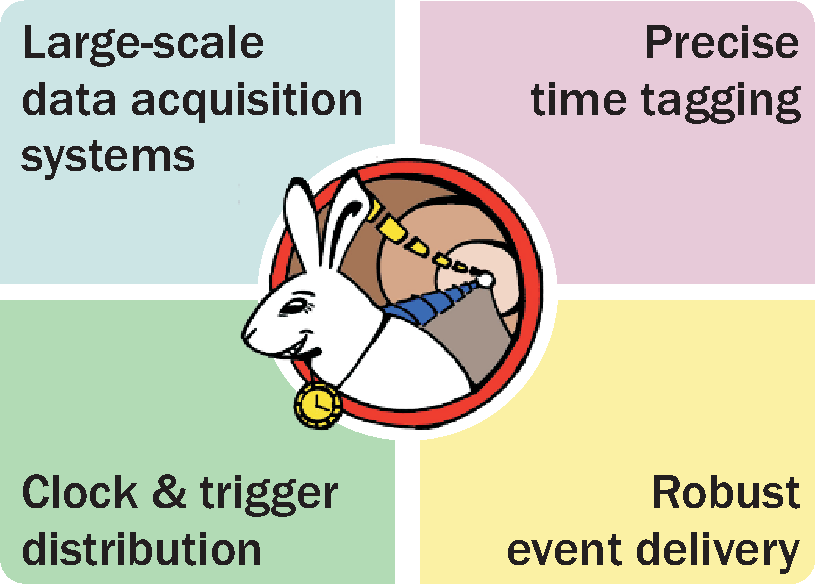
\includegraphics[width=7.5cm]{drawings/wr_apps.pdf}
\end{center}
\end{frame}


\subsection{WR in CERN's BE-CO-HT Hardware Kit}
\begin{frame}{WR in CERN's BE-CO-HT Hardware Kit}
\begin{center}

  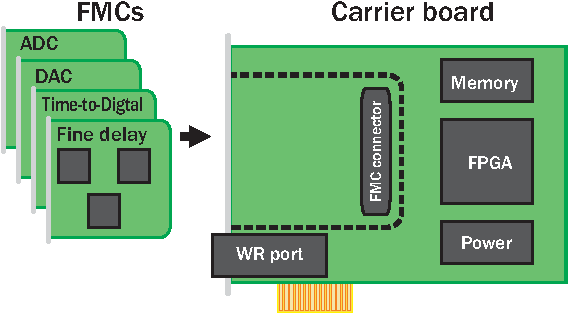
\includegraphics[width=6cm]{drawings/shw_kit}

  \begin{block}{CERN's BE-CO-HT FMC-based Hardware Kit:}
    \begin{itemize}
    \item FMCs (FPGA Mezzanine Cards) with ADCs, DACs, TDCs, fine delays, digital I/O.
    \item Carrier boards in PCI-Express, VME and uTCA formats.
    \item All carriers are equipped with a White Rabbit port.
    \end{itemize}
  \end{block}

\end{center}
\end{frame}


% \begin{frame}{Ethernet Clock distribution a.k.a. Distributed DDS}
%   \begin{center}
%     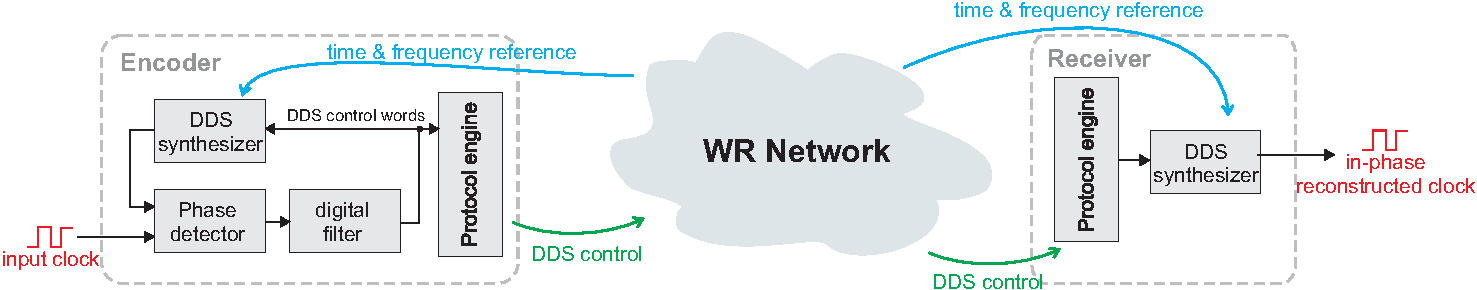
\includegraphics[width=\columnwidth]{drawings/remote_dds.pdf}
%   \end{center}
%   \begin{block}{Distributed Direct Digital Synthesis}
%     \begin{itemize}
%     \item Replaces dozens of cables with a single fiber.
%     \item Works over big distances without degrading signal quality.
%     \item Can provide various clocks (TTC, RF, bunch clock) with a single, standarized link.
%     \end{itemize}
%   \end{block}
% \end{frame}


\begin{frame}{Distributed oscilloscope}
  \begin{center}
    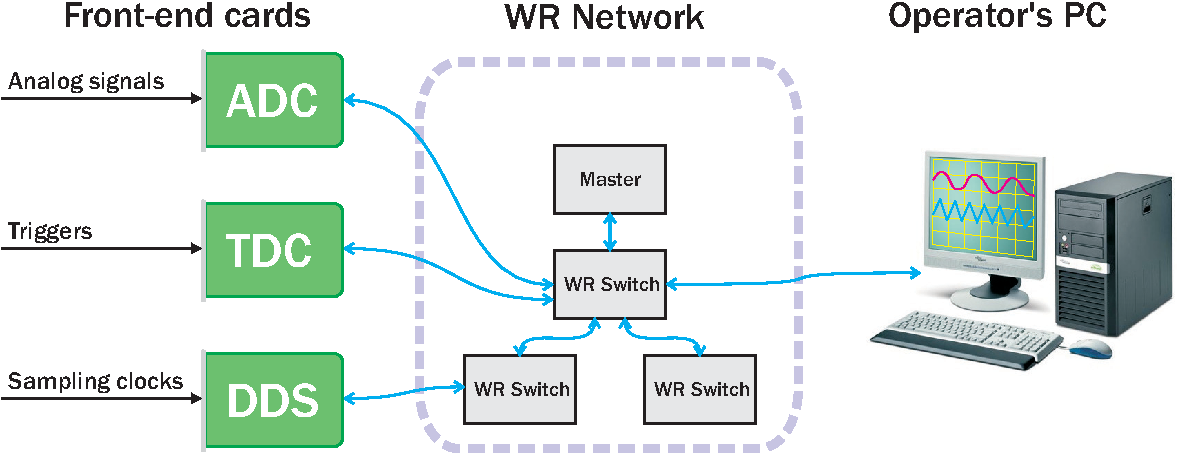
\includegraphics[width=8cm]{drawings/distr_oscill}
    \end{center}
    \begin{block}{}
      \begin{itemize}
      \item Common clock: no skew between ADCs
      \item Ability to sample with different clocks via Distributed DDS
      \item External triggers can be time tagged with a TDC and used to reconstruct the original time base in the operator's PC
      \end{itemize}
    \end{block}
\end{frame}



\section{Planning}

\subsection{Current status}

\begin{frame}{WR Switch development status}
	\begin{block}{Switch hardware}
          \begin{itemize}
            \item Working and debugged V2 hardware prototype
            \item Tested on 10-km fiber links
            \item Interoperates with standard Ethernet gear
            \end{itemize}
            \end{block}

	\begin{block}{Switch software}
          \begin{itemize}
            \item Done the Hardware Abstraction Layer and PTP daemon
            \item Sub-nanosecond accuracy over PTP has been achieved
            \item Verified interoperability with other PTP devices on ISPCS 2010 Plug Fest
            \end{itemize}
          \end{block}
\end{frame}

\begin{frame}{Already achieved...}
  \begin{block}{According to ISPCS Plug Fest results ...}
    \begin{center}
      \textbf{... White Rabbit is the most accurate PTP implementation in the world!}
  \end{center}
  \end{block}
\end{frame}

\subsection{Development plans for 2011}


\begin{frame}{Foreseen milestones}

  \begin{block}{WR Switch}
    \begin{itemize} 
      \item Basic functionality of HDL and software achieved, code cleanup underway
      \item V3 prototype (18 ports): Q4 2011
      \item Commercial product: Q2 2012 \\Estimated COTS price:
        $\sim$2500\euro
      \end{itemize}
    \end{block}

  \begin{block}{WR Ecosystem commercial availability}
    \begin{itemize} 
      \item PCIe carrier available now, VME Q2 2012
      \item WR timing node in VME and PCIe: Q2 2012
      \item Mezzanines: Full set of cards Q2 2012
      \end{itemize}
    \end{block}

\end{frame}

\begin{frame}{Summary}
  % Keep the summary *very short*.

\begin{block}{A deterministic timing and data link}
\begin{itemize}
\item 1 ns accuracy and 20 ps jitter
\item 10 km fiber links
\item Up to 2000 nodes
\end{itemize}
\end{block}

\begin{block}{A successful \textbf{open collaboration}}
\begin{itemize}
\item Fully open development
\item Involving institutes and companies
\item Full system commercially available mid-2012
\end{itemize}
\end{block}

\begin{center}
  For more information, \href{http://www.ohwr.org/projects/white-rabbit/wiki}{http://www.ohwr.org/projects/white-rabbit/wiki}    
\end{center}
\end{frame}

\end{document}
